Wiele nowoczesnych technologii i języków programowania udostępnia operacje na wektorach jako wydajniejszą i bardziej praktyczną alternatywę dla zwykłych działań na skalarach. Znajdują one zastosowanie w matematyce obliczeniowej, grafice komputerowej i innych dziedzinach wymagających wydajnych obliczeń na duzych tablicach danych. W bieżącym rodziale podajemy przykład zastosowania zaprojektowanego przez nas języka do rozwiązania zagadnień które mogą zostać wykorzystane w rzeczywistych problemach obliczeniowych.
\section{Ciąg fibonacciego}
Standardowe rozwiązanie problemu szukania \textit{n}-tego elementu ciągu fibonacciego polega na \textit{n}-krotnym dodaniu do siebie poprzednich elementów ciągu[1]. Zaproponowane przez nas rozwiązanie rozszerzone jest o szukanie 8 kolejnych elementów na raz. Warto zwrócić uwagę jak czytelne jest to rozwiązanie. Obliczony wynik jest zwracany poprzez ewaluacje przechowujące zmiennej w ostatniej linijce. Nie potrzebne jest żadne zarezerwowane słowo typu \textbf{return}. Poszczególne odpowiadające elementy wektorów są przez procesor dodawane w tym samym czasie dzięki czemu operacje na wektorach są tak samo szybkie jak na pojedynczych skalarach.\clearpage
\begin{lstlisting}[frame=single]
term1:IntVector[8] = [0,1,1,2,3,5,8,13]
term2:IntVector[8] = [1,1,2,3,5,8,13,21]
result:IntVector[8] = [0,0,0,0,0,0,0,0]

loop(5):
  result = term1 + term2
  term1 = term2
  term2 = result
end

result
#expecting [8, 13, 21, 34, 55, 89, 144, 233] 
\end{lstlisting}
\begin{figure}[H]
\centering
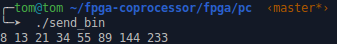
\includegraphics[scale=1]{images/fibb}
\caption{Rezultat wektorowego obliczania ciągu fibonacciego}
\end{figure}
Należy zauważyć, że takie rozwiązanie problemu prowadzi do wykonania nadmiarowej ilości operacji jako że każda wartość liczona jest kilkakrotnie jednak wektorowy charakter rozwiązania sprawia, że wiele z tych operacji wykonuje się jednocześnie.
\section{Rotacja figury w 3 wymiarach}
Operacja rotacji punktów jest zaproponowanym przez nas działaniem mającym pokazać rozszerzalność procesora o nowe mnemoniki. W swoim założeniu ma ona przyjmować 8 elementowy wektor składający się z 4 punktów po 2 współrzędne. Jej wynikiem ma być nowy wektor 8 elementowy zawierający 4 zadane punkty obrócone o 90 stopni względem punktu (128, 128). Funkcja \textbf{rot90} tłumaczona jest przez kompilator na asemblerową \textbf{RotS}. Sama rotacja względem punktu realizowana jest w sposób bardzo prosty. Jest ona złożeniem translacji do początku układu, rotacją względem punktu (0,0) (dzięki temu otrzymujemy bardzo prosty wzór) a na końcu znowu translacją - tym razem do punktu (128,128). Opisać ją można wzorem $rot90(x,y) = (256 - x, y) $. (Patrz rysunek 2.2)
\begin{figure}[!ht]
\centerline{
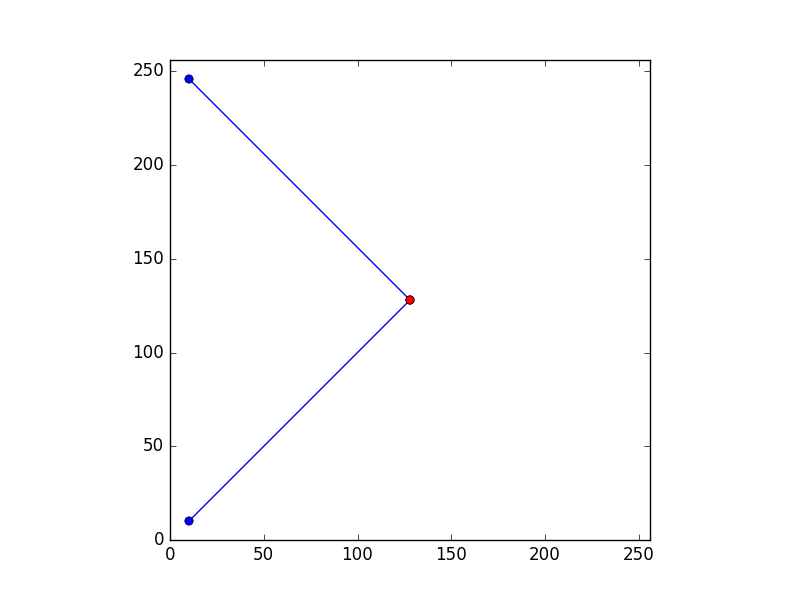
\includegraphics[scale=1]{images/figure_1}}
\caption{Rotacja niebieskiego punktu o 90 stopni względem czerwonego punktu (128, 128).}
\end{figure}
\clearpage
Zaproponowaną operacje możnaby wykorzystać na przykład do wizualizowania rotacji figur przestrzennych - wtedy 2 wektory mogłyby opisywać bryłę przed i po rotacji względem pionowej osi OZ.
\begin{lstlisting}[frame=single]
rot90 [10,10,100,10,90,90,30, 100]
 # result = [10, 246, 10, 156, 90, 166, 100, 226] 
rot90 [15,15,80,15,70,80,35,60]
 # result = [15,241,15,176,80,186,60,221] 
\end{lstlisting}
\begin{figure}[!ht]
\centerline{
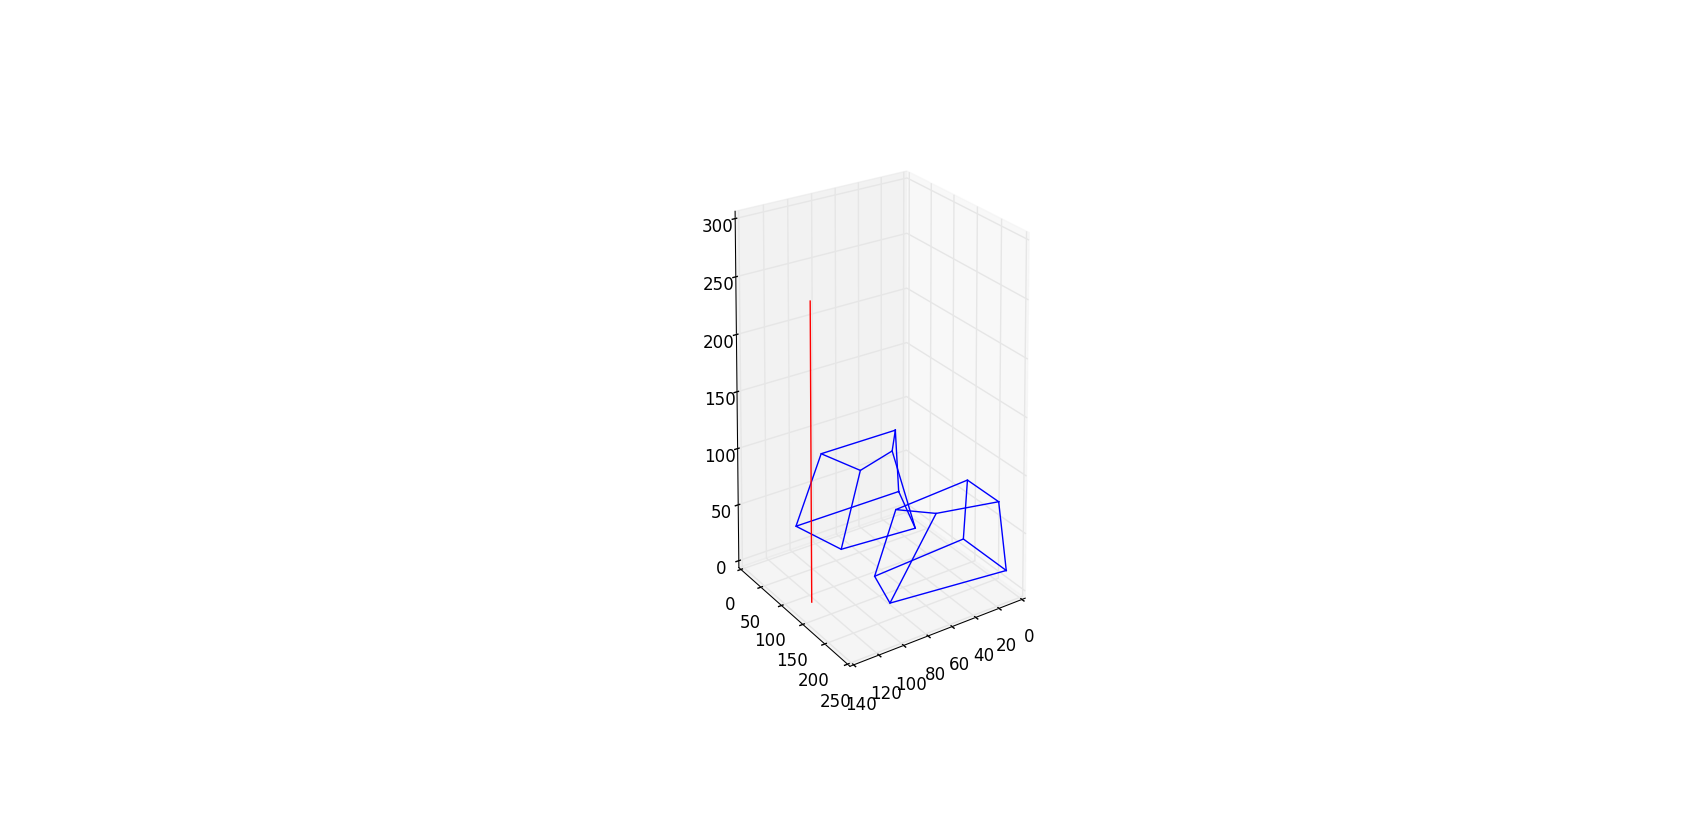
\includegraphics[scale=0.75]{images/3d_12}}
\caption{Figura i jej rotacja względem prostej równoległej do OZ i przechodzącej przez punkt (128, 128). Należy zwrócić uwagę, że wizualizacja przestrzeni trójwymiarowej nie oddaje w rzeczywisty sposób wszystkich kątów i odległości.}
\end{figure}
Rotacja o 90 stopni jest bardzo wydajna i prosta do wykonania gdyż nie wymaga operacji zmiennoprzecinkowych natomiast polega jedynia na zamianie miejsc współrzędnych (x,y) oraz odwróceniu znaku jednej z nich[2].
\section{Iloczyn skalarny}
Wprowadzenie do języka operacji iloczynu skalarnego umożliwia wykonanie wielu zadań z zakresu geometrii obliczeniowej[3]. Jednym z nich jest sprawdzenie prostopadłości dwóch wektorów. Co więcej, zmienna długość wektorów umożliwia sprawdzanie prostopadłości kąta w przestrzeniach wielowymiarowych.
\begin{figure}[!ht]
\centerline{
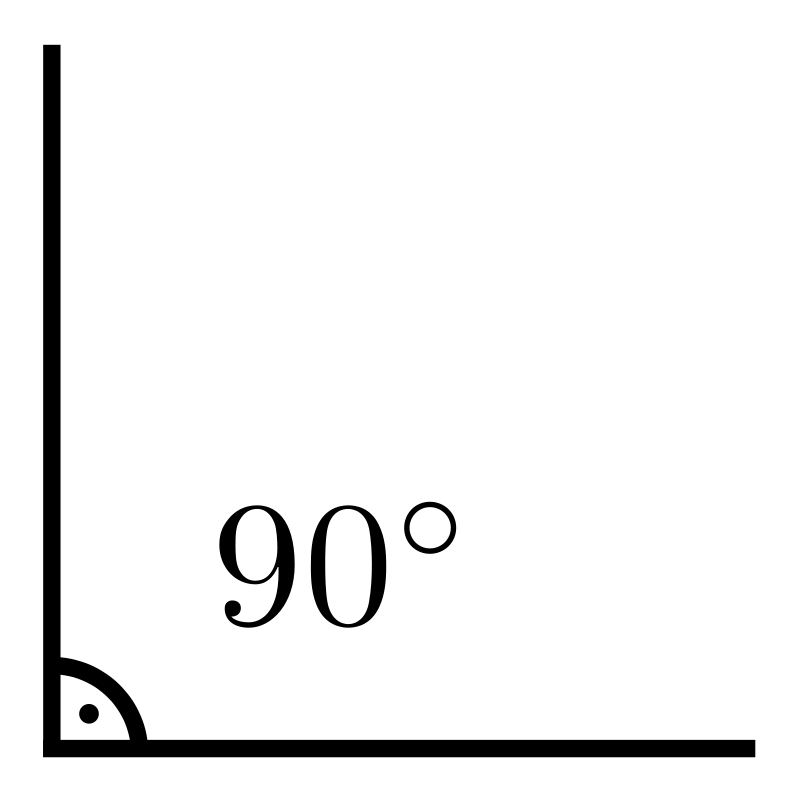
\includegraphics[scale=0.1]{images/kat_prosty}}
\caption{Kąt pomiędzy dwoma wektorami jest prosty jedynie wtedy gdy ich iloczyn skalarny jest równy zero.}
\end{figure}
\begin{lstlisting}[frame=single]
vec1:IntVector[4] = [1,3,0,5]
vec2:IntVector[4] = [0,0,10,0]
result:Int = vec1 ? vec2
result 
# wynik - 0: vec1 i vec2 sa prostopadle
\end{lstlisting}
Kolejnym zastosowaniem dla iloczynu skalarnego jest liczenie długości wektora w metryce euklidesowej zadanej wzorem:
$ d(x,y) = \sqrt{(\sum_{i=1}^{n} (x_i - y_i)^2}$. W aktualnym stadium projektu nie jest to możliwe z braku wsparcie dla operacji pierwiastka, jednak odległość definiowana jako różnica kwadratów może znaleźć zastosowanie na przykład gdy nie potrzebujemy znać dokładnych odległości a jedynie je porównywać pomiędzy różnymi punktami.

Iloczyn skalarny wraz z operacją pierwiastka może również zostać wykorzystany do liczenia cosinusa kąta pomiędzy wektorami:
$$ \cos{\theta} = \frac{ab}{\abs{a} \abs{b}} $$
Wzoru tego nie można w pełni wykorzystać podczas obliczeń na naszym procesorze, gdyż wymaga użycia liczb zmiennoprzecinkowych jednak daje on intuicje w jakim kierunko warto byłoby dalej rozwijać projekt.
\section{Wektorowa operacja modulo}
Wśród wspieranych przez nasz system operacji zarówno skalarnych jak i wektorowych jest funkcja \textit{modulo}[4]. Znajduje ona zastosowanie w wielu zadaniach z dziedziny teorii liczb, kombinatoryki oraz kryptografii. Może zostać wykorzystana do implementacji algorytmu znajdowania największego wspólnego dzielnika, najmniejszej wspólnej wielokrotności lub wyliczania rozwiązania dla chińskiego twierdzenia o resztach. W kryptografii używana jest do liczenia potęg modulo oraz logarytmowania dyskretnego.
Przykładowa operacja modulo element po elemencie: 
\begin{lstlisting}[frame=single]
a:IntVector[8] = [64, 7, 24, 1, 100, 125, 10, 2]
b:IntVector[8] = [8, 3, 16, 1, 15, 20, 5, 2]
result:IntVector[8] = a % b
result
# wynik [0, 1, 8, 0, 10, 5, 0, 0]
\end{lstlisting}
Modulo jest operacją powszechną we wszystkich popularnych językach programowania. Daje duże możliwości również na naszym procesorze, gdyż operuje on na liczbach całkowitych a więc może w pełni korzystać z danej operacji.